\documentclass{report}
\usepackage[T1]{fontenc} % Fontes T1
\usepackage[utf8]{inputenc} % Input UTF8
\usepackage[backend=biber, style=ieee]{biblatex} % para usar bibliografia
\usepackage{csquotes}
\usepackage[portuguese]{babel} %Usar língua portuguesa
\usepackage{blindtext} % Gerar texto automaticamente
\usepackage[printonlyused]{acronym}
\usepackage{hyperref} % para autoref
\usepackage{graphicx}

\bibliography{bibliografia}


\begin{document}
%%
% Definições
%
\def\titulo{Projeto 2}
\def\data{12 de junho de 2019}
\def\autores{João Oliveira, Bernardo Barreto,\\ Bernardo Falle, Diogo Vicente}
\def\autorescontactos{93282 joaoroliveira@ua.pt, 93271 @ua.pt,\\ 93331 mbfale@ua.pt, 93262 dvicente@ua.pt}
\def\versao{VERSAO 1}
\def\departamento{DEPARTAMENTO DE ELETRÓNICA TELECOMUNICAÇÕES E INFORMÁTICA}
\def\empresa{Universidade de Aveiro}
\def\logotipo{ua.pdf}
%
%%%%%% CAPA %%%%%%
%
\begin{titlepage}

\begin{center}
%
\vspace*{50mm}
%
{\Huge \titulo}\\ 
%
\vspace{10mm}
%
{\Large \empresa}\\
%
\vspace{10mm}
%
{\LARGE \autores}\\ 
%
\vspace{30mm}
%
\begin{figure}[h]
\center
\includegraphics{\logotipo}
\end{figure}
%
\vspace{30mm}
\end{center}
%
\begin{flushright}
\versao
\end{flushright}
\end{titlepage}

%%  Página de Título %%
\title{%
{\Huge\textbf{\titulo}}\\
{\Large \departamento\\ \empresa}
}
%
\author{%
    \autores \\
    \autorescontactos
}
%
\date{\data}
%
\maketitle

\pagenumbering{roman}

%%%%%% RESUMO %%%%%%
\begin{abstract}
Este projeto foi feito com o intuito de ganharmos mais conhecimentos na parte de programação em python tal como na utilização de HTML , protocolos HTTP, API's, entre uma serie de outras coisas.
O objetivo final do trabalho era fazer uma pagina web que fosse possivel ser visualizada uma galeria de fotos, e fazer uma vasta pesquisa de acordo com vários argumentos que utilizador quisesse utilizar, podendo estes ser RGB, nome do objeto, nivel de confiança. Com isto realizamos codigo em pyhton utilizando a biblioteca da cherryPy criando assim um servidor para que fosse possivel estabelecer uma ligaçao entre a nossa database e o nosso site. Na parte de HTML foi utilizado todo o procedimento normal e após isto a utilização do css e do js. O primeiro para dar style ao nosso site, tornando assim mais \textit{user friendly} e também com um aspeto melhor. O JavaScript foi usado para criar funções obtendo assim valores de diferentes sliders, etc... para depois podermos utilizar isto no nosso código e obter os resultados que o utilizador pretende. A identificação de objetos e de cores domintantes utilizadas como metodo de pesquisa no site são obtidas utilizando também o nosso código em Python juntamente com a máquina fornecidas pelos docentes da cadeira. Tornando assim um site completamente funcional e que identifica diversos objetos. 
\end{abstract}

%%%%%% Agradecimentos %%%%%%
% Segundo glisc deveria aparecer após conclusão...
\renewcommand{\abstractname}{Agradecimentos}
\begin{abstract}
Agradecer aos colegas que sempre se disponibilizaram para ajudar. E um especial agradecimento a todos os docentes da cadeira que nos ajudaram em todas as nossas dúvidas.
\end{abstract}


\tableofcontents
% \listoftables     % descomentar se necessário
% \listoffigures    % descomentar se necessário


%%%%%%%%%%%%%%%%%%%%%%%%%%%%%%%
\clearpage
\pagenumbering{arabic}

%%%%%%%%%%%%%%%%%%%%%%%%%%%%%%%%
\chapter{Introdução}
\label{chap.introducao}

Este relatório foi criado com o propósito de ir ao encontro com os objetivos mencionados no segundo projeto realizado no âmbito da unidade curricular de Laboratórios de Informática. O relatório primeiramente irá sofrer de uma breve apresentação introdutória, após isto teremos todas as fases fundamentais do projeto divididas por capitulos, por fim temos uma breve conclusão acerca do projeto.

Para este projeto foi-nos proposto que realizassemos um sistema que permita visualizar uma biblioteca de imagens com suporte para a procura e a identificação dos objetos contidos nas bibliotecas armazenadas, pode ser todo o tipo de coisas como, pessoas, automoveis, bancos, animais, etc.. Desta forma temos uma máquina disponibilizada pelos docentes da disciplina, que identifica estes objetos. Após isto foi-nos colocado o desafio de criar numa linguagem, à nossa escolha, nos optamos por python, um programa que relacionado com um site pode-se de facto dar-nos a biblioteca de imagens como foi proposto inicialmente.

O relatório será divido de acordo com as diferentes componentes do trabalho em capitulos, e subcapitulos que irão explicar devidamente todos os procedimentos e cuidados que tivemos ao realizar este trabalho. Este será o primeiro capitulo em que obtemos uma pequena introdução teórica do trabalho. Prontamente começamos com a explicaçao do \autoref{chap.Front-end}, após isto iremos falar da \autoref{chap.Base de dados} explicando como funciona seguido do \autoref{chap.Servidor} e concluindo com a \autoref{chap.Interligação} destes todos.




\chapter{Front-end}
\label{chap.Front-end}

Na parte de Front-end, focamo-nos a usar html, css e js. \\
No css usamos o bootstrap que nos ajudou com todas as classes para que podessemos dar style ao projeto de maneira a que este ficassse esteticamente melhor e mais organizado. Javascript usamos algumas funções de modo a que conseguissemos retirar valores do nosso slider, por exemplo.

\section{HTML}
Nesta secção foi onde escrevemos todo o código HTML relativamente ao nosso site, esquematizando assim todas as páginas necessárias e o que nelas continha. Temos assim cinco ficheiros .html, em que cada um deles corresponde a uma pagina do site. O primeiro ficheiro corresponde à nossa home em que temos a nossa galeria apresentada, na segunda pagina o utilizador pode fazer uma pesquisa de imagem de acordo com o nivel de confiança, na terceira damos a hipotese de o utilizador dar upload a uma imagem para o nosso servidor que será guardada e depois apresentada na nossa galeria, na quarta será possivel pesquisar pelo objeto e pela devida cor dominante da imagem, na quinta temos apenas a informação básica de todos os membros do projeto assim como a divisão do trabalho. Tudo isto realizado na linguagem HTML com ajuda de JS e CSS que iremos explicar o porquê de seguida.
\section{CSS}
Na parte do CSS tivemos ajuda do bootstrap que nos facultou diversas classes, o que facilitou muito a parte de style do projeto. Também criamos ficheiros de css criados por nós para dar style a nossa galeria de fotos, e a outros objetos que preferimos fazer de raiz.

\section{JS}
No JavaScript utilizamos pouco, apenas realizamos pequenas funções que nos facultavam valores que depois poderiamos utilizar nos programas atrás para niveis de confiança, por exemplo.

\chapter{Base de Dados}
\label{chap.resultados}
A base de dados construída na linguage SQL contém uma tabela \textit{images} que tem 5 campos de informação
\subsection{ID}
É o campo mais simples, sendo que é o tipo \textit{integer primary key auto increment}, isto é, cada vez que é feito o upload de uma imagem para o site o \textit{id} incrementa automaticamente.
\subsection{Classe}
Este elemento da tabela é o nome do objeto extraído da imagem original que sofreu upload. Este nome é obtido através do JSON que é fornecido pela máquina do Docente João Paulo Barraca.
\subsection{Original hash}
Este campo é o nome que nos é dado pelo ficheiro existente que está armazenado nas pastas de storage (storage/objects) que contém as imagens originais. Este nome já vem encriptado do cherryPy.
\subsection{Image hash}
Este elemento da tabela é a designação da imagem já recortada com as coordenadas definidas pela máquina anteriormente descrita. Este Image hash contém sempre o mesmo nome (cropped) e depois, dependendo dos números de objetos extraídos, aumenta o número apresentado a seguir. Assim o nome da imagem recortada com um objeto vai ser, por exemplo: \texttt{cropped\_0\_OriginalHash}.
\subsection{Confidence}
Este membro da tabela vai buscar a confiança da máquina fornecida e redirecciona para o elemento \textit{Confidence} da base de dados. Para esclarecimento, a confiança da imagem é a percentagem de certeza que o objeto extraído é, de facto, o objeto dado pela máquina.
\subsection{Color}
O último componente da tabela é o elemento Color, e é redireccionado de uma função feita pelos responsáveis por este tema. Este componente regista a cor predominante (red, green, blue) de cada objeto extraído. De seguida, armazena na base de dados.

\chapter{Servidor}
CherryPy é uma \textit{web framework} do Python que através dela conseguimos utilizar facilmente uma interface para um protocolo HTTP. Também pode ser chamada de \textit{web application library}.\\
O cherryPy tira proveito da linguagem dinamica do Python para passar o protocolo HTTP para uma API. O que fornece uma plataforma de confiança.

\subsection{Statics}
De modo a que o servidor consiga mostrar os conteúdos estáticos é necessário a utilização de um dicionário, \textit{config}, que remete para as respetivas pastas destes conteúdos. O dicionário é depois utilizado ao dar \textit{mount}.

\subsection{Classes}
\subsubsection{List}
Esta classe contém apenas um método chamado de index. Este método possui 3 argumentos que conforme os seus valores vão dar \textit{return} a diferentes funções da \textit{database}.
Essas funções dão return a objetos JSON.
\subsubsection{Get}
Apenas contém uma função index, e como argumento o id. Esta função conforme o id passado irá devolver uma imagem completa.
\subsubsection{Put}
Esta classe também só possui uma função index que recebe um ficheiro como argumento, passando-a para \textit{hash} em MD5, após isto a função irá guardar o ficheiro no server que postiormente manda para uma função na database que processa a imagem. Seguidamente reencaminha o utilizador para a página onde se encontrava.
\subsubsection{Root}
A root é a função que serve o conteúdo HTML ao utilizador. Possui cinco funções correspondentes às cinco páginas do site. Tem também uma função de inicialização das outras classes. Esta classe root é a classe central que serve de raiz para o servidor.


\chapter{Análise}
\label{chap.analise}
Analisando todos os objetivos, e fazendo uma recolha de testes podemos comprovar que no nosso trabalho apesar da maioria das funções funcionar, não conseguimos por a funcionar corretamente a listagem tanto de fotos como de nomes de objetos.\\
Segue também fotos de testes utilizados no site:

\begin{figure}
  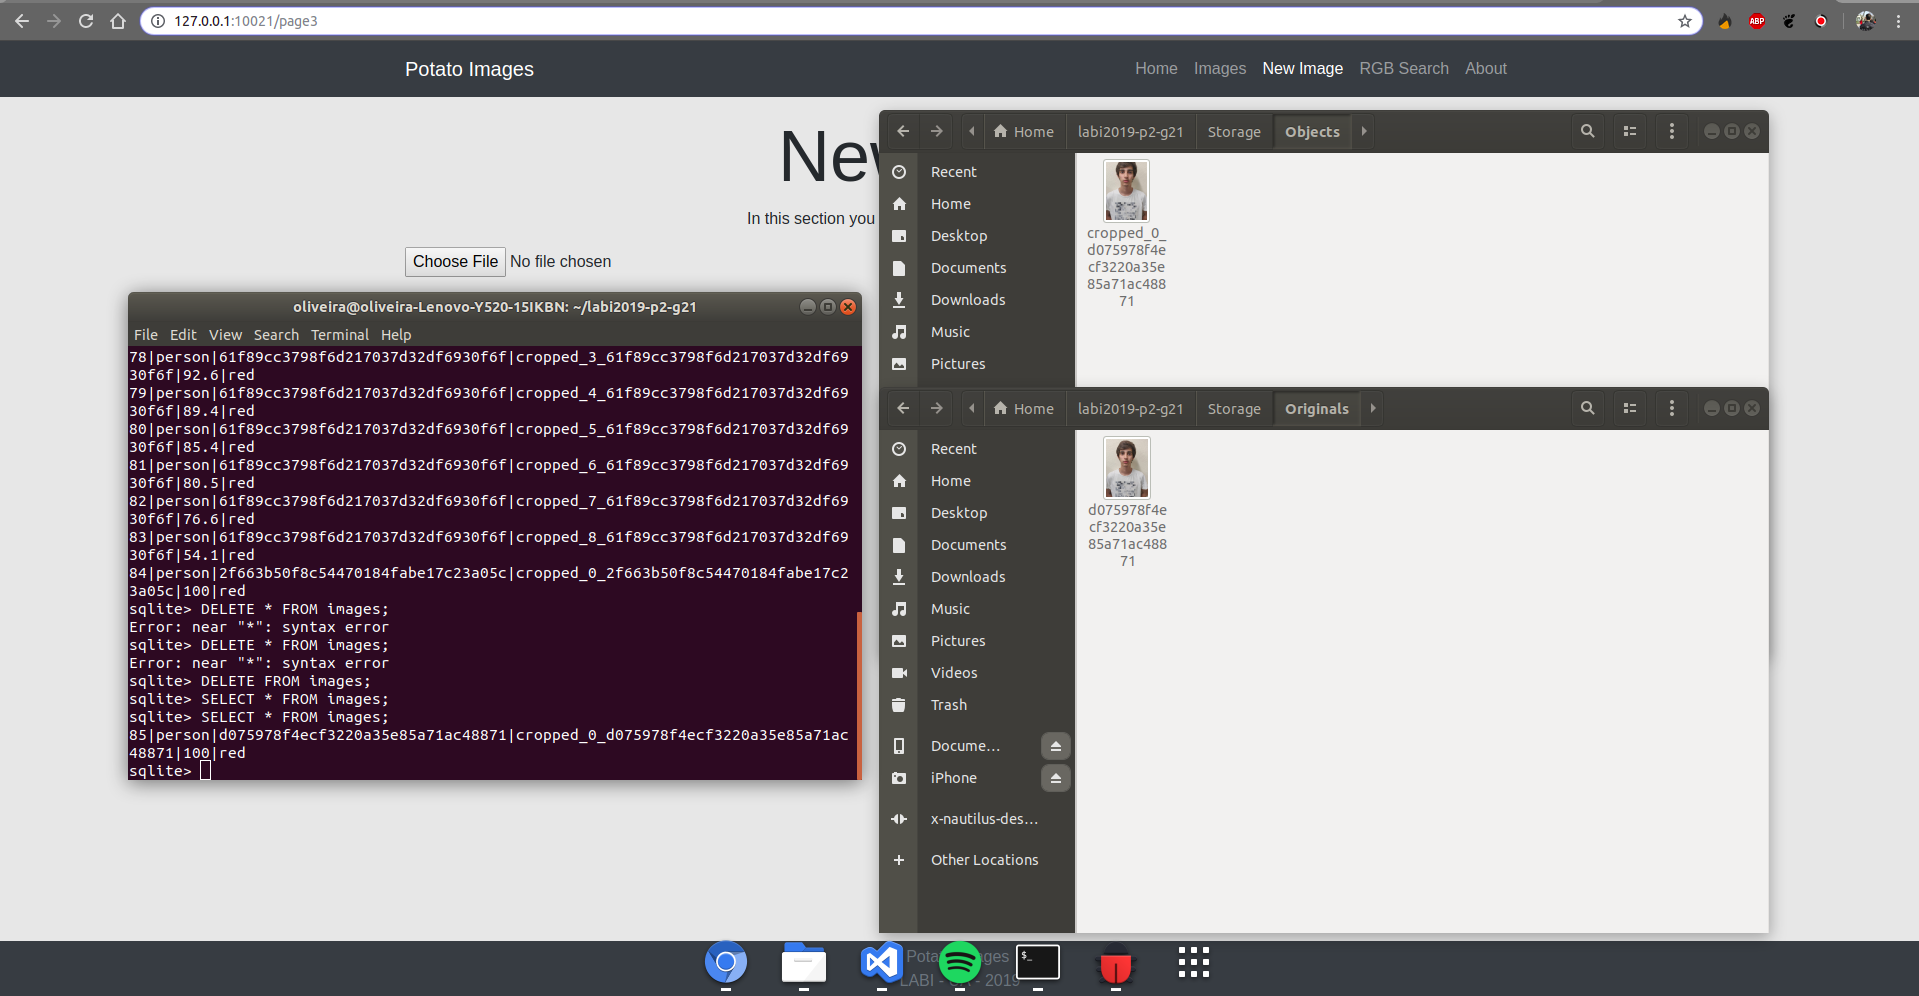
\includegraphics[width=\linewidth]{teste1.png}
  \caption{teste de adição de foto.}
  \label{teste de adição de foto}
\end{figure}

\begin{figure}
  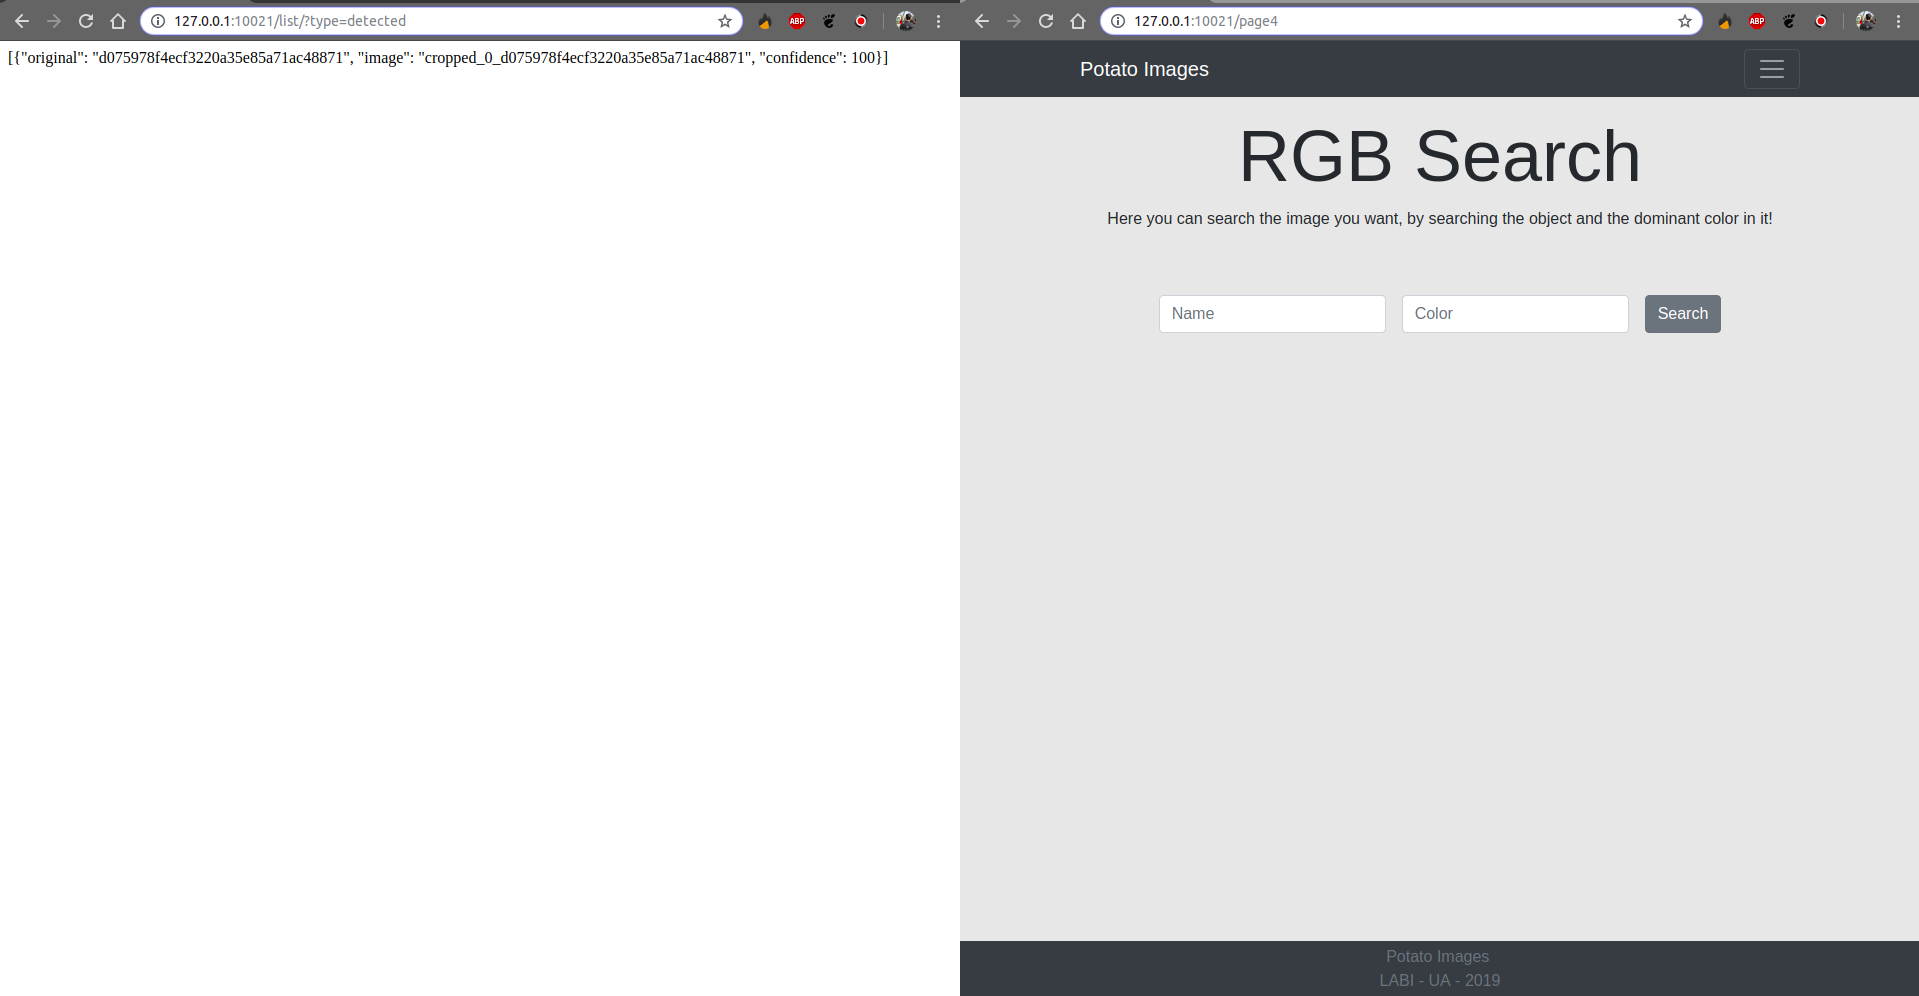
\includegraphics[width=\linewidth]{teste2.png}
  \caption{teste de verificação da cor e do objeto.}
  \label{teste de verificação da cor e do objeto}
\end{figure}



\chapter{Conclusões}
\label{chap.conclusao}
Concluindo este projeto, verificamos que apesar de conseguir fazer grande parte do projeto tivemos bastantes dificuldades em certas funções e em certas funcionalidades deste.
Sendo algumas destas analisadas no capítulo acima, tendo assim também testes que comprovam o que está a funcionar corretamente e o que não está.

\chapter*{Contribuições dos autores}
O \ac{JO} tratou da maior parte da front-end. \\
O \ac{BB} tratou da maior parte dos requests.\\
O \ac{DV} tratou da maior parte do servidor.\\
O \ac{BF} tratou da maior parte da base de dados.\\
Apesar desta divisão todos os membros tiveram sempre em conjunto a fazer o trabalho ajudando-se mutuamente em todo o código realizado neste projeto, sendo assim a divisao da percentagem de contribuição de 25\% para todos os membros.

%%%%%%%%%%%%%%%%%%%%%%%%%%%%%%%%%
\chapter*{Acrónimos}
\begin{acronym}
\acro{ua}[UA]{Universidade de Aveiro}
\acro{miect}[MIECT]{Mestrado Integrado em Engenharia de Computadores e Telemática}
\acro{lei}[LEI]{Licenciatura em Engenharia Informática}
\acro{glisc}[GLISC]{Grey Literature International Steering Committee}
\acro{JO}[JO]{João Oliveira}
\acro{BB}[BB]{Bernardo Barreto}
\acro{DV}[DV]{Diogo Vicente}
\acro{BF}[BF]{Bernardo Fale}
\end{acronym}


%%%%%%%%%%%%%%%%%%%%%%%%%%%%%%%%%
\printbibliography

\end{document}